\section{Introduction}\label{sec:ggtt_intro}
The cross section for the simultaneous production of a pair of Higgs bosons (di-Higgs production) at the LHC has a SM prediction of about 35\fb at $\sqrtS=13$\TeV~\cite{LHCHiggsCrossSectionWorkingGroup:2016ypw}. This is three orders of magnitude lower than the cross section for the production of a single Higgs boson, and as such, makes the search for di-Higgs production exceedingly difficult. Nevertheless, the CMS and ATLAS collaborations have performed these searches~\cite{CMS:2024awa,CMS-PAS-HIG-20-011,ATLAS:2024ish} and while they have not discovered di-Higgs production yet, they still act as important tests of the SM. One of the LO Feynman diagrams for di-Higgs production, shown in \cref{fig:dihiggs_feynman} (left), includes the $\PH\PH\PH$ vertex, thereby allowing these searches to place direct constraints on the Higgs self-coupling, $\lambda$, or alternatively on $\kappa_\lambda = \lambda / \lambda_{\text{SM}}$.

\begin{figure}
  \centering
  \inputtikz{Figures/Dihiggs/introduction/hh.tex} \hspace{1cm}
  \inputtikz{Figures/Dihiggs/introduction/res.tex}
  \caption[LO Feynman Diagrams for Nonresonant and Resonant Di-Higgs Production]{Examples of LO Feynman diagrams for nonresonant (left) resonant (right) di-Higgs production. In the resonant diagram, \PY is a new scalar.}\label{fig:dihiggs_feynman}
\end{figure}

The type of di-Higgs production in the SM is \textit{nonresonant}, meaning that it does not proceed via an intermediate resonance. In some BSM theories, di-Higgs production can proceed via new resonances (\textit{resonant} production), with a rate substantially higher than the SM prediction. An example for resonant production is shown in the Feynman diagram in \cref{fig:dihiggs_feynman} (right). In the WED and NMSSM theories described in \cref{sec:wed,sec:susy}, the possible resonant processes include \XZeroHH and \XTwoHH, where \XZero and \XTwo are new spin-0 and spin-2 particles, respectively, and \XYH, where \PX and \PY are new spin-0 particles. To gain a complete understanding of di-Higgs production at the LHC, it is important to search for both resonant and nonresonant production, and for a particular final state, the two are often done in parallel.

\begin{figure}
  \centering
  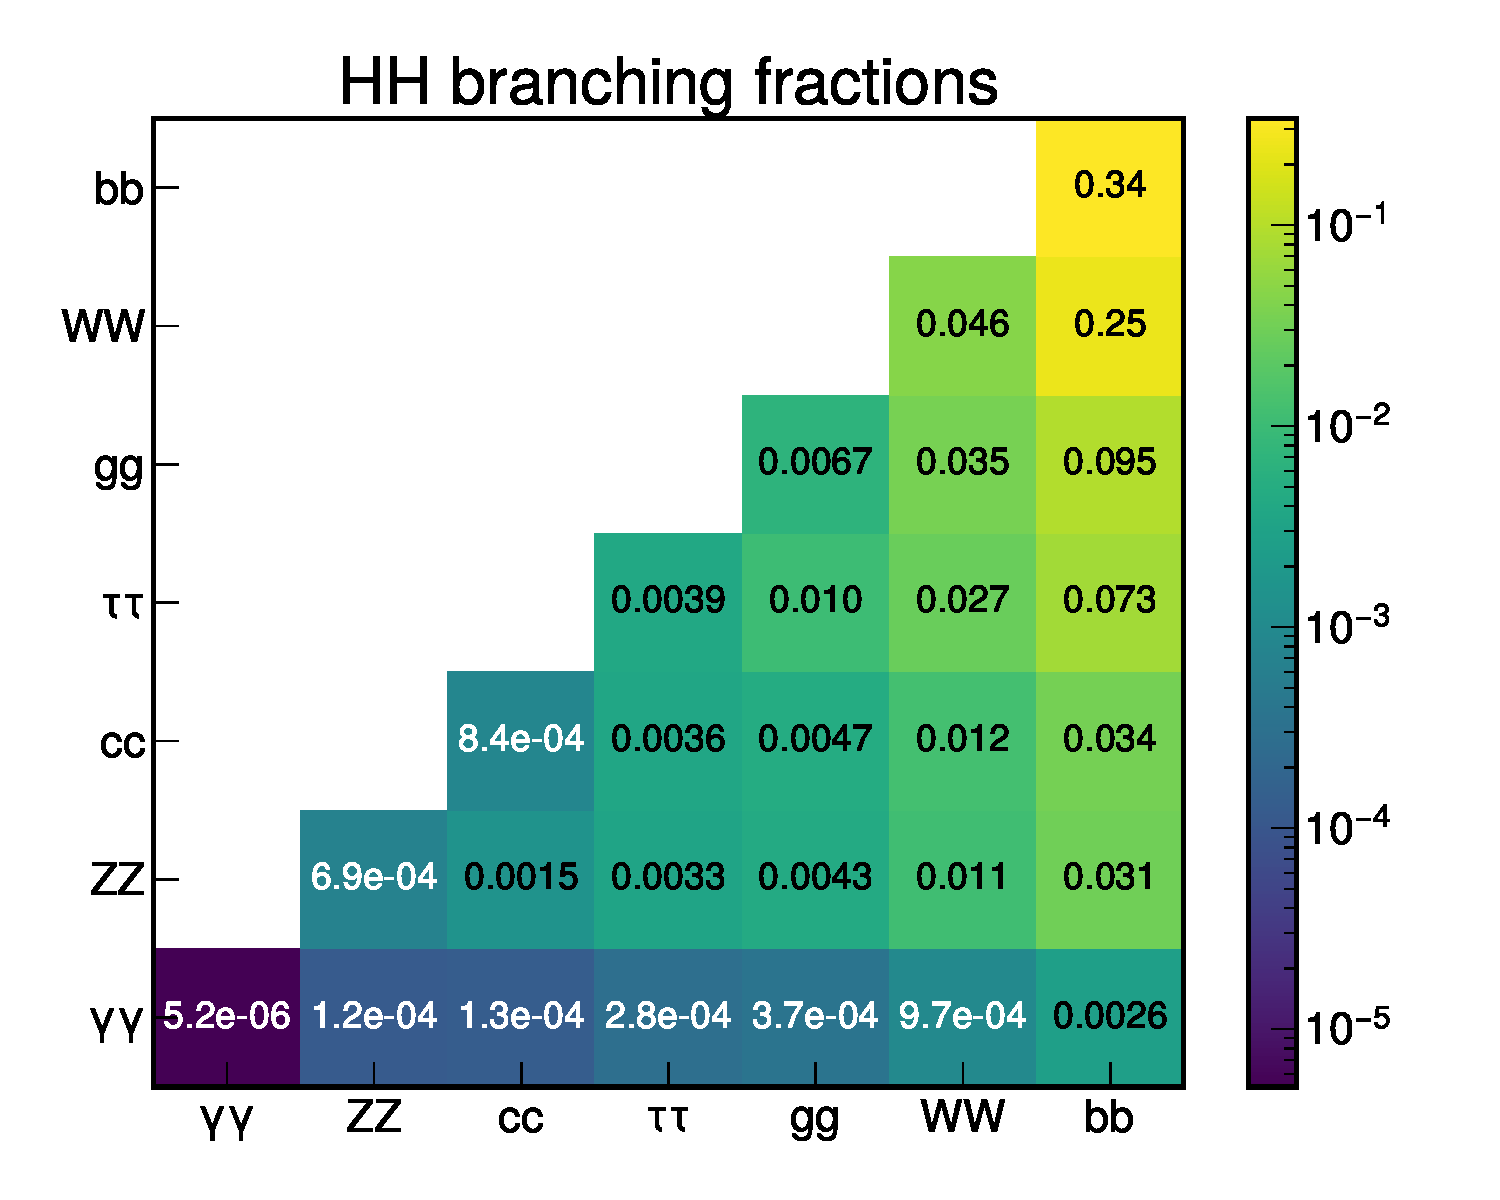
\includegraphics[width=0.7\textwidth]{Figures/Dihiggs/introduction/dihiggs_br.pdf}
  \caption[SM Di-Higgs Branching Fractions]{Branching fractions of \HH to different final states in the SM. For example, $\BR(\HH \to \ggtt) = 2.8\times10^{-4}$.}\label{fig:dihiggs_br}
\end{figure}

In designing a search for di-Higgs production, one must select which final states to use. To maximize sensitivity, it is important to choose a final state that has a combination of a high branching fraction, high signal efficiency, and low background contamination. \Cref{fig:dihiggs_br} shows the \HH branching fractions for the most common Higgs boson decays. The $\PH\PH \to b\bar{b}b\bar{b}$ decay has the highest branching fraction at 33\% but suffers from a large QCD multi-jet background, and relatively poor resolution on the reconstructed Higgs boson mass. By substituting one of the $b\bar{b}$ decays with $\gamma\gamma$, background levels are greatly reduced, and the analysis benefits from the good \mgg resolution. This makes the $\PH\PH \to b\bar{b}\gamma\gamma$ decay one of the most sensitive channels for \HH production at the LHC, despite its lower branching fraction of 0.26\%.

Searches for nonresonant and resonant di-Higgs production in the \bbgg final state have been performed by the CMS experiment with data from proton-proton collisions at $\sqrtS=13$\TeV corresponding to an integrated luminosity of 138\fbinv~\cite{CMS:2020tkr,CMS:2023boe}. The nonresonant search observed an upper limit on $\sigma(pp \to \HH \to \bbgg)$ of 5.2 times the SM prediction, and constrained the Higgs self coupling to $-3.3 < \kl < 8.5$~\cite{CMS:2020tkr}. The resonant search explored \XHH and \XYH production, with $\mX \in [260, 1000]$\GeV and $\mX \in [300, 1000]$\GeV respectively. In \XYH production, the \Ybb decay with $\mY \in [70, 800]$\GeV was considered. In the \XHH searches, no significant deviations from the background-only hypothesis were observed, and upper limits on $\sigma(pp \to \PX \to \HH \to \bbgg)$ were reported as 0.82--0.07 and 0.87--0.06\fb depending on \mX for the spin-0 and spin-2 scenarios respectively. In the \XYH search, an excess with a local (global) significance of 3.8 (2.8) standard deviations was observed at $\mX=650$\GeV and $\mY=90$\GeV~\cite{CMS:2023boe}. All upper limits and confidence intervals were set at 95\% CL.

The excess at $\mX=650$\GeV and $\mY=90$\GeV in the \XYH search is particularly interesting because it aligns with several others excesses reported by the CMS experiment. Searches for new scalars decaying to \WW, $\tau\tau$, and $\gamma\gamma$ final states have reported local (global) significances of 3.8 (2.6), 2.8 (2.2) and 2.9 (1.3) standard deviations for scalar masses of 650\GeV, 100\GeV and 95\GeV respectively~\cite{CMS:2022bcb,CMS:2022goy,CMS:2024yhz}. Assuming that these excesses are real and hint toward a new particle sector, they imply that $\sigma(\XYH)$ and decay rates of the new scalars to $b\bar{b}$, \WW, $\tau\tau$, and $\gamma\gamma$ are high enough to be observed (or almost observed) at the LHC. 

This motivates a search for \XYH production in the \ggtt final state, which has not been explored yet. Furthermore, for low values of \mY ($\sim 100\GeV$) in the \Ygg search, this analysis provides a unique opportunity to constrain regions of the NMSSM phase space, as discussed in \cref{sec:low_mass_in_NMSSM}. In the \XHH searches, the results are not expected to be more sensitive than those reported by the \bbgg search since the \Htautau branching fraction is lower than for \Hbb, but the search is motivated nonetheless by a future combination of results that will use all available final states to search for \XHH production with greater sensitivity than the individual analyses.

This chapter presents a search for resonant di-Higgs production in the \ggtt final state using proton-proton collision data collected by the CMS experiment between 2016 and 2018 at $\sqrtS=13$\TeV, corresponding to an integrated luminosity of 138\fbinv. The search consists of four main analyses, each targeting a different process:
\begin{enumerate}
  \item \XZeroHH: resonant \HH production via a spin-0 particle (\XZero) 
  \item \XTwoHH: resonant \HH production via a spin-2 particle (\XTwo)
  \item \XYttHgg: resonant $\PY\PH$ production via a scalar, \PX, where \Ytt
  \item \XYggHtt: resonant $\PY\PH$ production via a scalar, \PX, where \Ygg
\end{enumerate}
For the \XHH searches, $\mX \in [260, 1000]\GeV$, and for the \XYH searches, $\mX \in [300, 1000]$\GeV and $\mY \in [50, 800]$, where in the \XYggHtt search, the lower bound on \mY is instead 70\GeV due to triggering requirements. While these processes are motivated by the WED and NMSSM theories, the searches are designed to be model-independent, except for the assumption that the new particles have a narrow width. The final results are significances in the case of signal excesses, and upper limits on the cross section of the targeted processes. 



